\documentclass{beamer}

% --- Pacotes essenciais (seguros com o tema SINTEF) ---
\usepackage[T1]{fontenc}
\usepackage[utf8]{inputenc} % remova se compilar com XeLaTeX/LuaLaTeX
\usepackage[portuguese]{babel}
\usepackage{lmodern}
\usepackage{amsmath,amsfonts}
\usepackage{oldgerm} % você já usava; pode remover se não precisar

% --- Tema e fontes ---
\usetheme{sintef}
\usefonttheme[onlymath]{serif}

% --- Macros do seu template/exemplos ---
\newcommand{\testcolor}[1]{\colorbox{#1}{\textcolor{#1}{test}}~\texttt{#1}}
\newcommand{\hrefcol}[2]{\textcolor{cyan}{\href{#1}{#2}}}

% --- Title background (versão estrelada, antes do \maketitle) ---
\titlebackground*{assets/background}

% --- Bibliografia: mostrar número do item ---
\setbeamertemplate{bibliography item}{\insertbiblabel}

% --- Metadados ---
\title{Attention Models: da motivação às variantes modernas}
\subtitle{Intuição geométrica, formulação matemática e aplicações}
\author{Rodrigo Petrus Domingues, Felipe Grael e Vivian}
\date{\today}

\begin{document}

\maketitle

% ============================
% Evolução: LSTM → Atenção → Transformer (apenas frames)
% ============================

\section{Motivação e Histórico}


\begin{frame}{Redes Neurais Recorrentes}

	\begin{figure}[h]
		\centering
		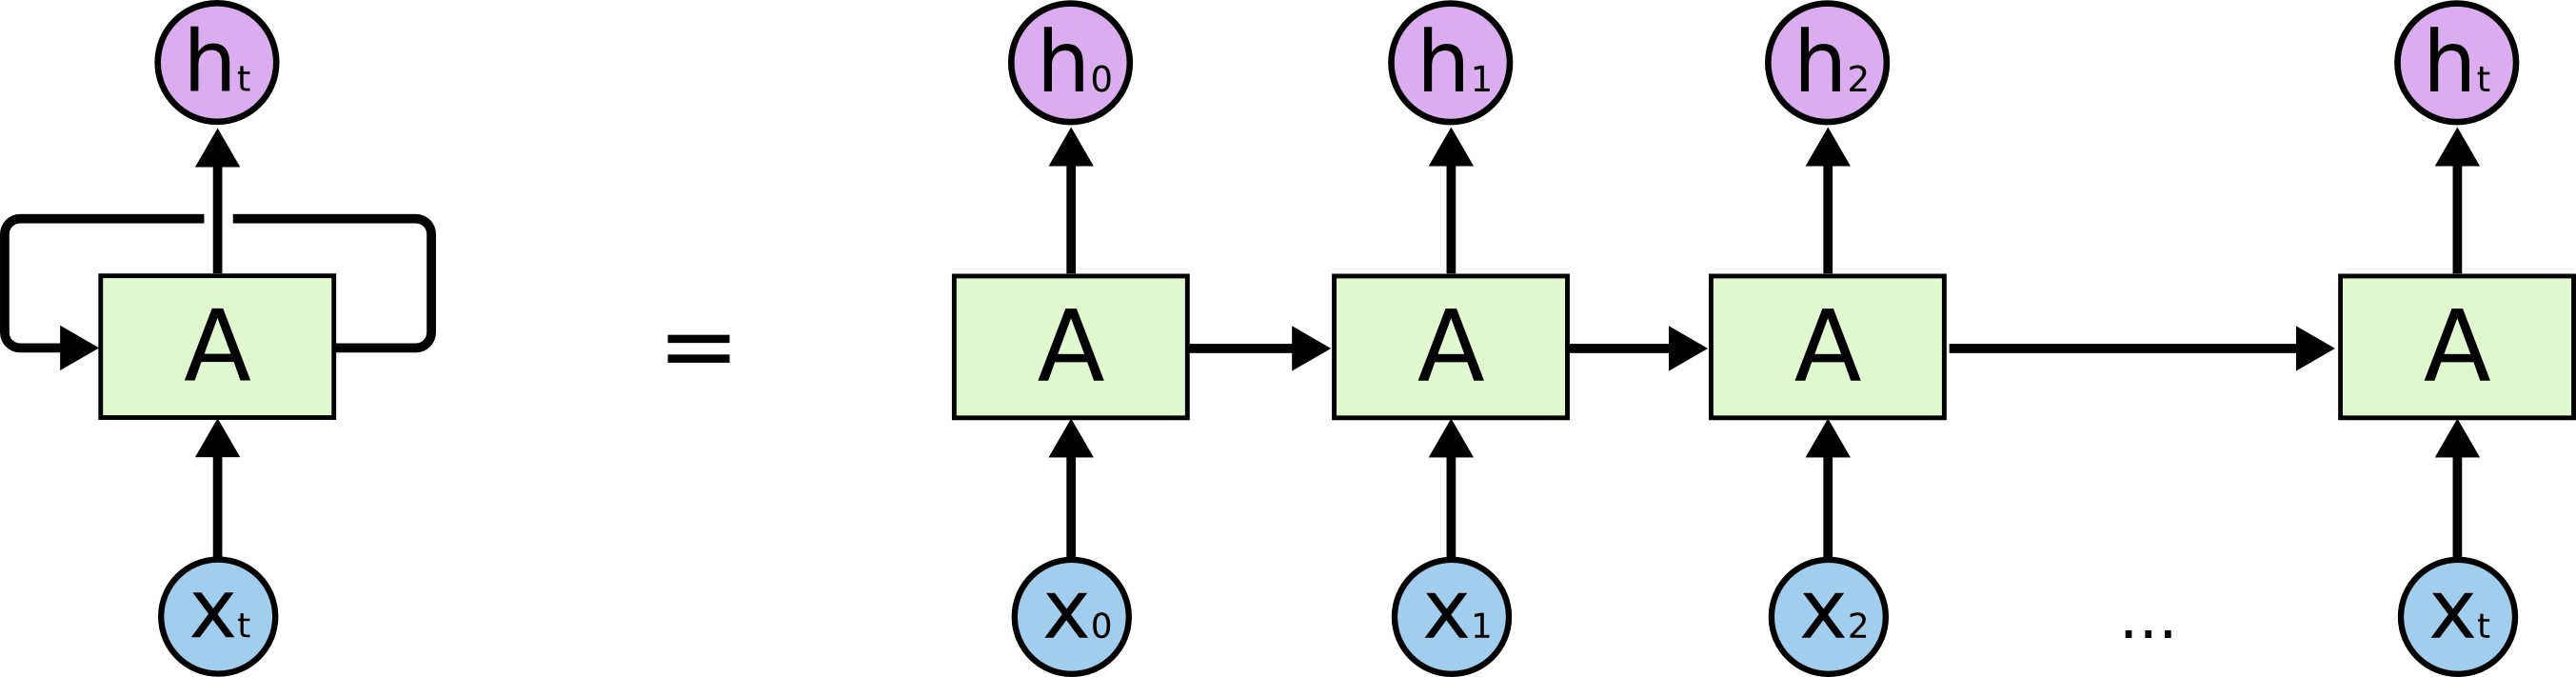
\includegraphics[width=0.6\textwidth]{assets/colah-RNN-unrolled.png}
		\caption{Redes Neurais Recorrentes \footnote{Figura de \href{https://colah.github.io/posts/2015-08-Understanding-LSTMs/}{Christopher Olah}}}
	\end{figure}

	\begin{itemize}
		\item Bem adaptadas para dados sequenciais como séries temporais e texto
		\item Diferentes tipos de modelos: LSTM, GRU
		\item Diferentes arquiteturas: simples, bidirecional, encoder-decoder
	\end{itemize}

\end{frame}

\begin{frame}{Tipos de camadas RNN}
	\begin{columns}[t]
		\column{0.5\textwidth}
		\vspace{-5mm}
		\begin{center}
			\textbf{LSTM}
		\end{center}
		\vspace{-5mm}
		\begin{figure}[h]
			\centering
			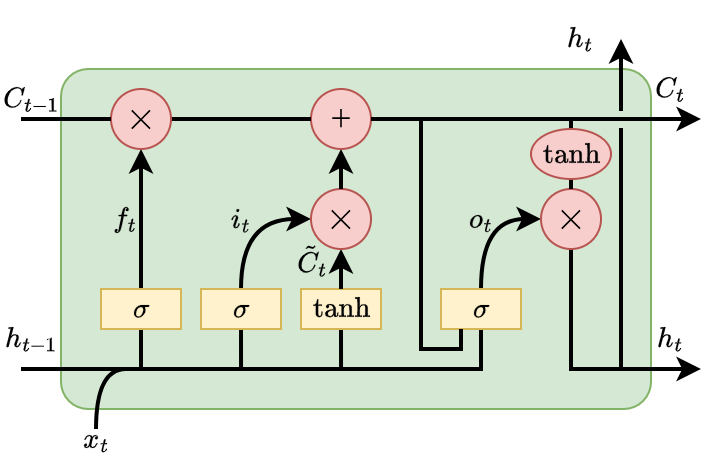
\includegraphics[width=0.5\textwidth]{assets/LSTM_Gates.png}
		\end{figure}
		\vspace{-2mm}
		\tiny
		\[
		\begin{alignedat}{2}
			f_t & = \sigma(W_f [h_{t-1}, x_t] + b_f), \quad & 
			i_t & = \sigma(W_i [h_{t-1}, x_t] + b_i), \\
			\tilde{C}_t & = \tanh(W_c [h_{t-1}, x_t] + b_c), \quad &
			C_t & = f_t \odot C_{t-1} + i_t \odot \tilde{C}_t, \\
			o_t & = \sigma(W_o [h_{t-1}, x_t] + b_o), \quad &
			h_t & = o_t \odot \tanh(C_t)
		\end{alignedat}
		\]
		\column{0.5\textwidth}
		\vspace{-5mm}
		\begin{center}
			\textbf{GRU}
		\end{center}
		\vspace{-5mm}
		\begin{figure}[h]
			\centering
			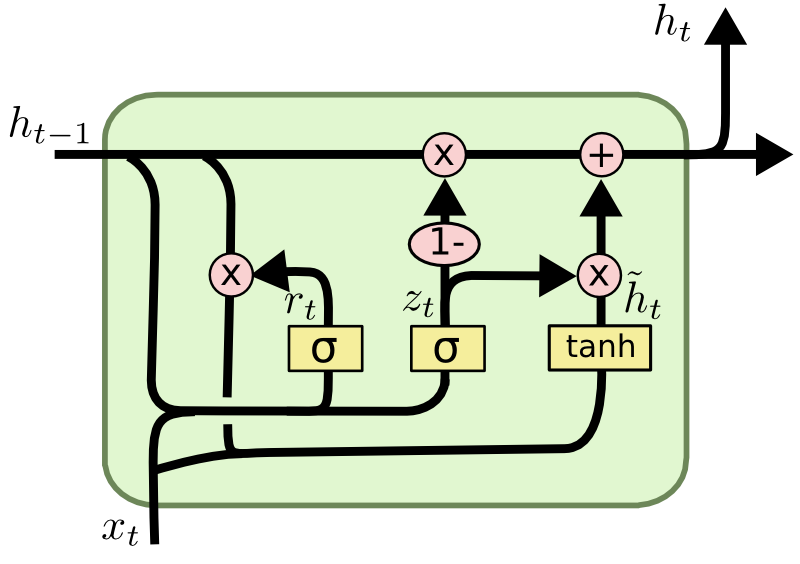
\includegraphics[width=0.5\textwidth]{assets/colah-GRU-layer.png}
		\end{figure}
		\vspace{-2mm}
		\tiny\[
			\begin{aligned}
				z_t         & = \sigma(W_z \cdot [h_{t-1}, x_t ])               \\
				r_t         & = \sigma(W_r \cdot [h_{t-1}, x_t ])               \\
				\tilde{h}_t & = \tanh(W \cdot [r_t \odot h_{t-1}, x_t ])        \\
				h_t         & = (1 - z_t) \odot h_{t-1} + z_t \odot \tilde{h}_t
			\end{aligned}
		\]

	\end{columns}
\end{frame}

\begin{frame}{Arquitetura Seq2Seq para Tradução}
	\begin{figure}
		\centering
		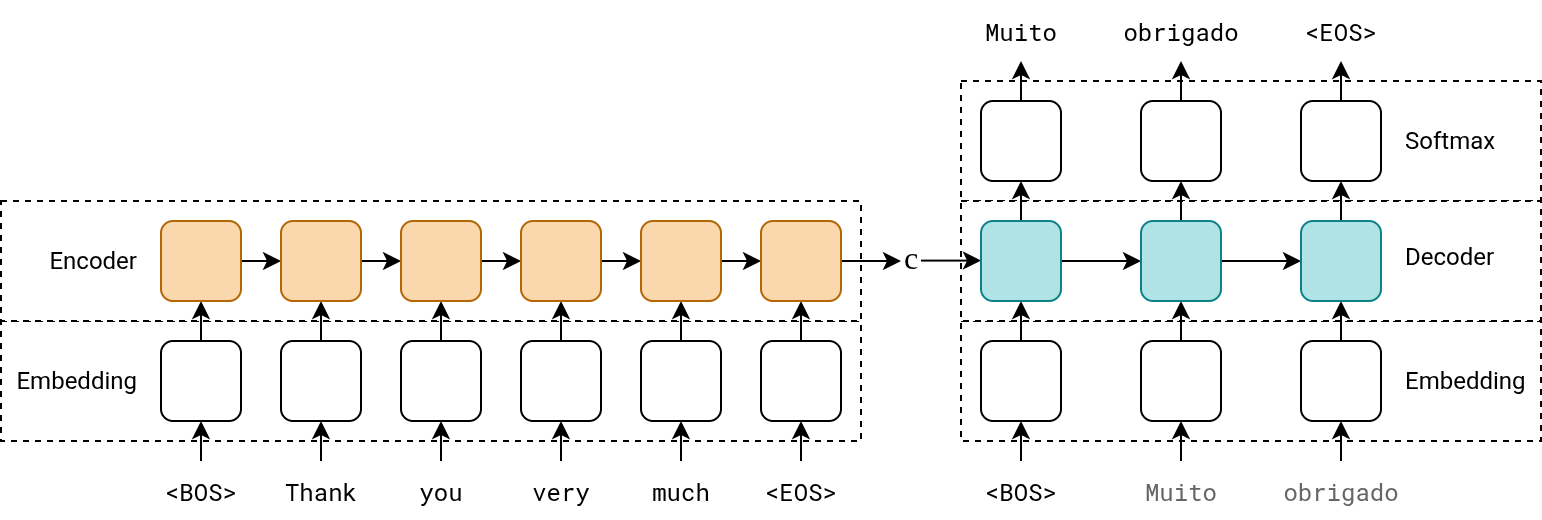
\includegraphics[width=0.7\textwidth]{assets/Seq2Seq_NMT.png}
	\end{figure}
	\begin{itemize}
		\item \textbf{Gargalo}: toda a informação comprimida em $c=h_n$.
		\begin{itemize}
			\item Processamento \textbf{sequencial} $\Rightarrow$ baixa paralelização.
			\item \textbf{Dependências longas} ainda são difíceis (mesmo com portas).
			\item \textbf{Gargalo do contexto} (vetor único) degrada qualidade em frases longas.
		\end{itemize}
	\end{itemize}
\end{frame}

% 3) Solução 1: Atenção sobre o encoder (Bahdanau/Luong)
\begin{frame}{Atenção aditiva \cite{bahdanau2014neural}}
\[
e_{ij} = a(s_{i-1}, h_j), \quad
\alpha_{ij} = \frac{\exp(e_{ij})}{\sum_{k=1}^{T_x} \exp(e_{ik})}, \quad
c_i = \sum_{j=1}^{T_x} \alpha_{ij} h_j
\]

\begin{itemize}
  \item $h_j$: estado oculto do encoder na posição $j$ (palavra $x_j$).
  \item $s_{i-1}$: estado do decoder no passo anterior ($y_{i-1}$).
  \item $e_{ij}$: escore de alinhamento entre $h_j$ e $s_{i-1}$ (via rede feedforward).
  \item $\alpha_{ij}$: pesos normalizados (softmax) $\to$ distribuem a atenção sobre os $h_j$.
  \item $c_i$: vetor de contexto dinâmico usado para prever $y_i$.
\end{itemize}

\textbf{Intuição:} O decoder calcula, em cada passo, um mapa de atenção sobre os estados do encoder, decidindo onde focar.
\end{frame}

\begin{frame}{Integração com encoder bidirecional e decoder}
\begin{itemize}
  \item O \textbf{encoder} é uma RNN bidirecional:
  \[
  h_j = [\overrightarrow{h_j}; \overleftarrow{h_j}]
  \]
  Cada $h_j$ contém contexto passado e futuro da palavra $x_j$.
  
  \item O vetor de contexto $c_i$ é construído a partir desses estados bidirecionais.
  
  \item O \textbf{decoder} (RNN unidirecional) atualiza seu estado com:
  \[
  s_i = f(s_{i-1}, y_{i-1}, c_i)
  \]
  - Usa o estado anterior $s_{i-1}$
  - O símbolo anterior $y_{i-1}$
  - O contexto dinâmico $c_i$
  
  \item Assim, a cada passo, o decoder combina memória interna + contexto dinâmico para prever $y_i$.
\end{itemize}

\textbf{Resultado:} 
Resolve o gargalo do vetor fixo único ($h_n$) e permite traduções mais fiéis em frases longas.
\end{frame}


\begin{frame}{Atenção multiplicativa \cite{luong2015effective}}
\textbf{Três variantes de scoring:}
\[
\begin{aligned}
e_{ij} &= v^\top \tanh(W [s_j; h_i]) && \text{(concat, similar ao Bahdanau)} \\
e_{ij} &= s_j^\top W h_i && \text{(general)} \\
e_{ij} &= s_j^\top h_i && \text{(dot)}
\end{aligned}
\]

\begin{itemize}
  \item $s_j$: query → estado oculto do decoder.
  \item $h_i$: key/value → estado do encoder.
  \item \textbf{Concat:} aproxima-se da atenção aditiva de Bahdanau.
  \item \textbf{General:} bilinear, mais expressivo (aprende $W$).
  \item \textbf{Dot:} mais simples e rápido (nenhum parâmetro extra).
\end{itemize}

\textbf{Nota:} Podemos reinterpretar em termos modernos como $Q=s_j$, $K=h_i$, $V=h_i$.
\end{frame}

\begin{frame}{Global vs Local Attention \cite{luong2015effective}}
\begin{columns}[c]
  \column{0.35\textwidth}
    \begin{figure}
      \centering
      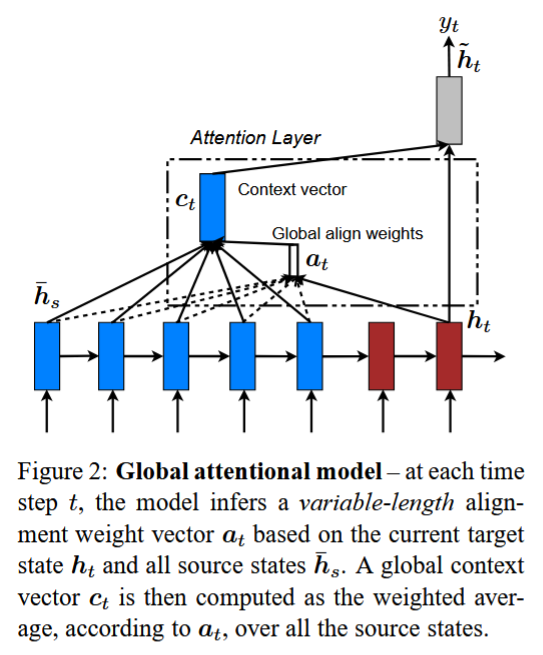
\includegraphics[width=\linewidth]{assets/global attention.png}
      \caption*{Global Attention}
    \end{figure}
  \column{0.35\textwidth}
    \begin{figure}
      \centering
      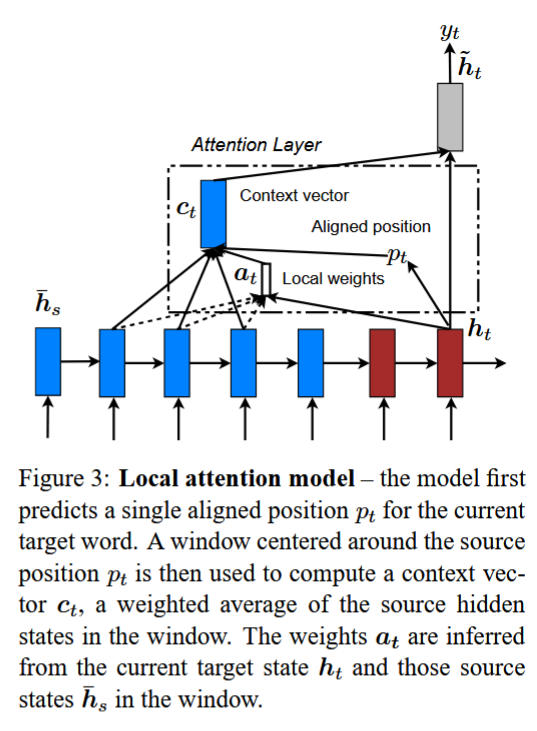
\includegraphics[width=\linewidth]{assets/local attention.png}
      \caption*{Local Attention}
    \end{figure}
\end{columns}

\begin{itemize}
  \item \textbf{Global:} o decoder olha para \emph{todos} os estados do encoder em cada passo $j$.  
  \item \textbf{Local:} o decoder olha apenas para uma \emph{janela limitada} de estados do encoder ao redor de uma posição prevista $p_t$.  
  \item O cálculo do contexto $c_j$ é o mesmo, mas a diferença está no \textbf{escopo de atenção}.  
\end{itemize}

\textbf{Resumo:}  
Global é mais expressivo mas caro; Local é mais eficiente e pode capturar alinhamentos monotônicos mais naturalmente.
\end{frame}


% 4) Solução 2: Self-Attention (intra-sequência)
\begin{frame}{Self-Attention: dependências em paralelo}
	\[
		\mathrm{Att}(Q,K,V)=\mathrm{softmax}\!\left(\frac{QK^\top}{\sqrt{d_k}}\right)V,
		\quad
		Q = XW_Q,\; K = XW_K,\; V = XW_V.
	\]
	\begin{itemize}
		\item Calcula relações \emph{entre todos os tokens} da mesma sequência, \textbf{em paralelo}.
		\item Multi-head:
		      \[
			      \mathrm{MHA}(X)=\mathrm{Concat}(H_1,\dots,H_h)\,W_O,\quad
			      H_r=\mathrm{softmax}\!\left(\frac{Q_r K_r^\top}{\sqrt{d_k}}\right)V_r.
		      \]
		\item Comparativo: RNN/LSTM exige $n$ passos sequenciais; self-attention faz um passo paralelo com custo $\mathcal{O}(n^2)$.
	\end{itemize}
\end{frame}

\begin{frame}{Arquitetura pré-transformer}
\begin{figure}
  \centering
  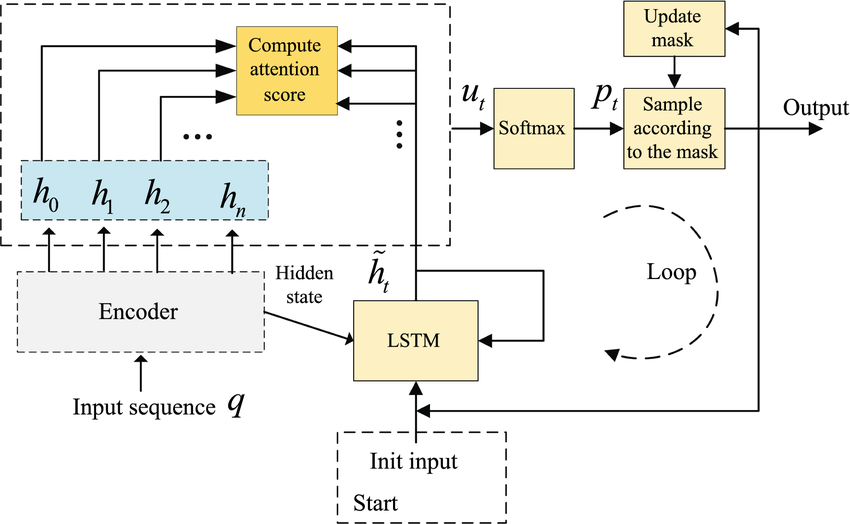
\includegraphics[height=0.75\textheight]{assets/The-framework-of-additive-attention-mechanism-in-decoder.png}
  \caption{Exemplo de arquitetura pré-transformer (aditiva) \cite{gu2022pointer}}
\end{figure}
\end{frame}

\section{Transformers}
% 5) Transformer: tirar LSTM, adicionar posição + FFN e empilhar blocos
\begin{frame}{Attention Is All You Need \cite{vaswani2017attention}: nascendo o Transformer}
	\begin{itemize}
		\item \textbf{Remove} completamente a recorrência (sem LSTM).
		\item \textbf{Positional encodings} preservam ordem:
		      \[
			      PE_{(pos,2i)}=\sin\!\left(\frac{pos}{10000^{2i/d_{\text{model}}}}\right),\quad
			      PE_{(pos,2i+1)}=\cos\!\left(\frac{pos}{10000^{2i/d_{\text{model}}}}\right).
		      \]
	\end{itemize}
	\begin{figure}
	\centering
	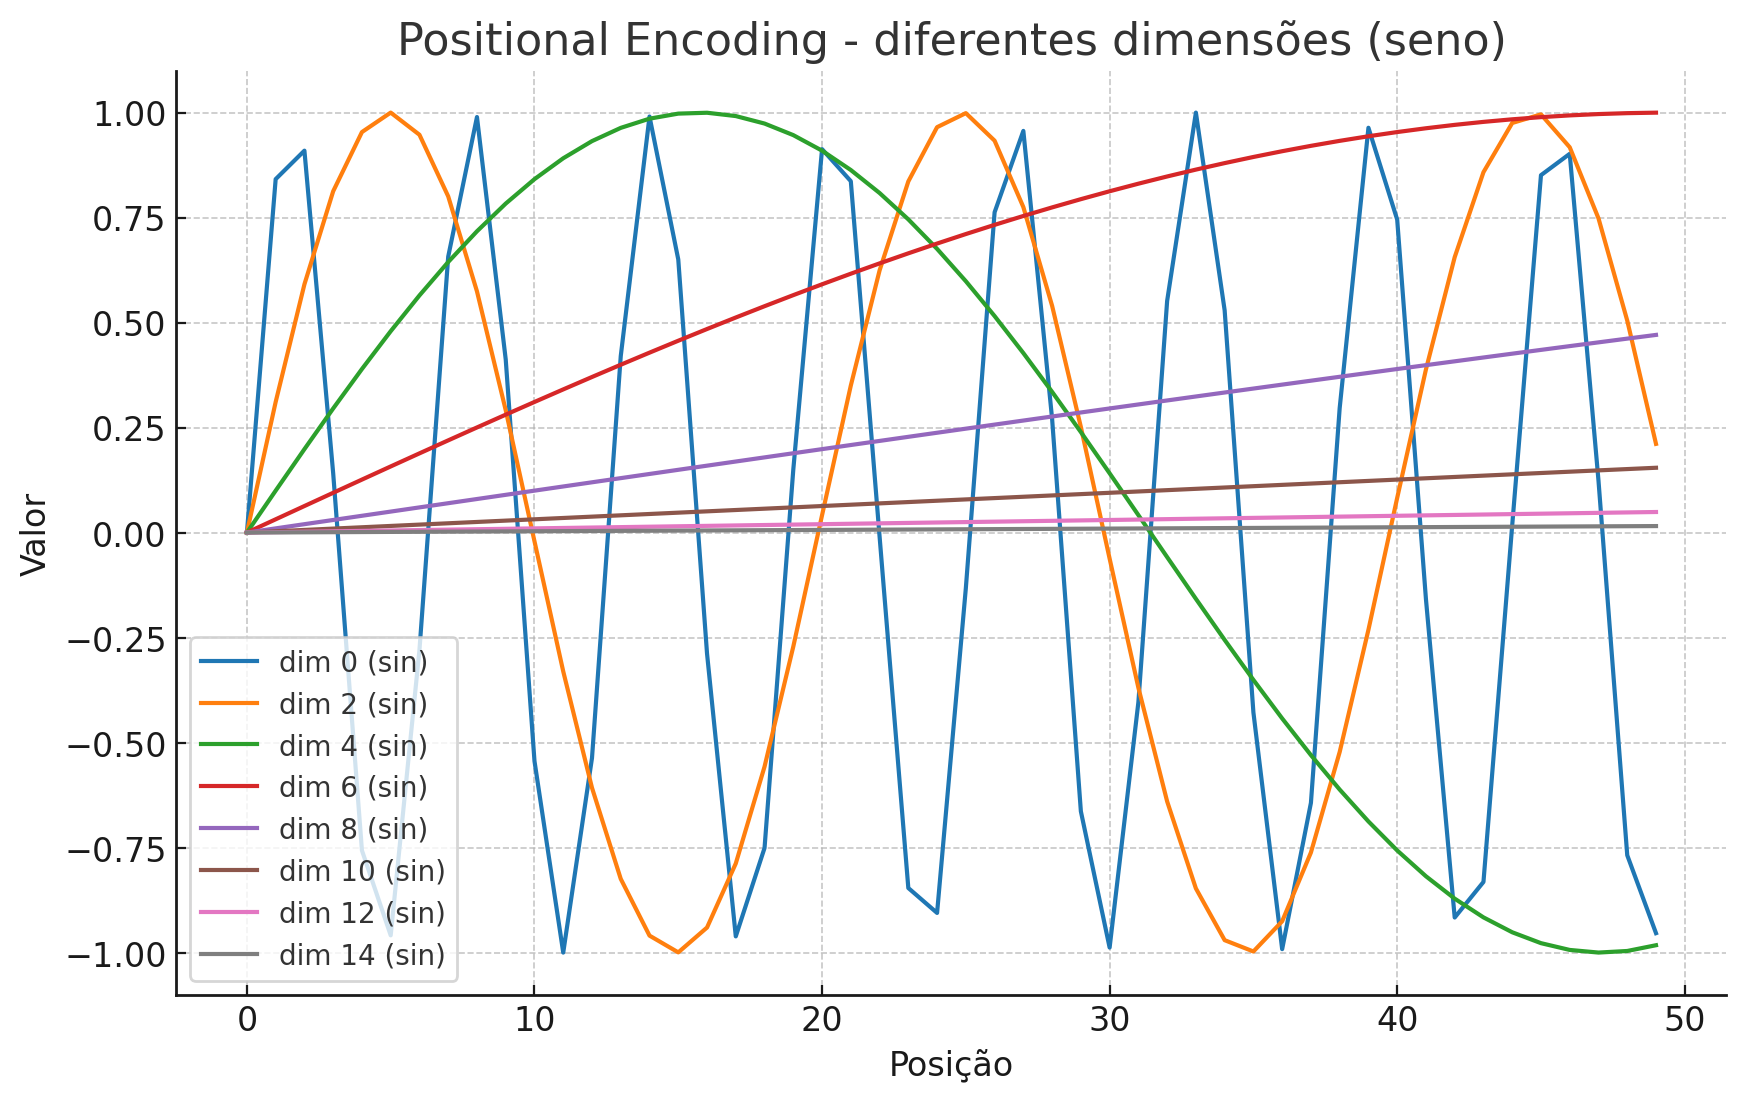
\includegraphics[height=0.55\textheight,width=0.7\linewidth]{assets/positional-encoding.png}
	\caption{Exemplo de codificação posicional senoidal \cite{vaswani2017attention}}
	\end{figure}	
\end{frame}

\begin{frame}{Bloco Transformer e arquitetura}
	\begin{itemize}
		\item Cada \textbf{bloco Transformer} (pré-norm, forma comum):
		      \[
			      \begin{aligned}
				      Y & = X + \mathrm{MHA}(\mathrm{LN}(X)),                                               \\
				      Z & = Y + \mathrm{FFN}(\mathrm{LN}(Y)),\quad \mathrm{FFN}(u)=W_2\,\phi(W_1u+b_1)+b_2,
			      \end{aligned}
		      \]
		\item Empilha-se vários blocos de atenção+FFN $\Rightarrow$ \textbf{arquitetura Transformer}.
	
		\item \textbf{Máscara causal} (para LMs) impede olhar o futuro:
		\[
			\mathrm{softmax}\!\left(\frac{QK^\top}{\sqrt{d_k}}+M\right),
			\quad
			M_{ij}=\begin{cases}
				0,       & j\le i \\
				-\infty, & j>i
			\end{cases}
		\]
	\end{itemize}
\end{frame}

\begin{frame}{Arquiteturas Transformer e Aplicações}
\begin{columns}[t]
  % Coluna 1
  \column{0.33\textwidth}
  \textbf{Encoder--Decoder} \\
  (Transformer original, 2017)
  \begin{itemize}
    \item Tradução automática
    \item Sumarização
    \item Diálogo
    \item Captioning
  \end{itemize}

  % Coluna 2
  \column{0.33\textwidth}
  \textbf{Encoder-only} \\
  (BERT, RoBERTa, DistilBERT)
  \begin{itemize}
    \item Classificação de texto
    \item NER (entidades)
    \item QA (extração de trechos)
    \item Análise semântica
  \end{itemize}

  % Coluna 3
  \column{0.33\textwidth}
  \textbf{Decoder-only} \\
  (GPT, LLaMA, etc.)
  \begin{itemize}
    \item Modelos de linguagem
    \item Geração de texto
    \item Completamento de prompts
    \item Story generation
  \end{itemize}
\end{columns}
\end{frame}

\begin{frame}{Arquiteturas Transformer: encoder e decoder \cite{vaswani2017attention}}
\begin{columns}[t]	
	\column{0.33\textwidth}
	\begin{figure}
		\centering
		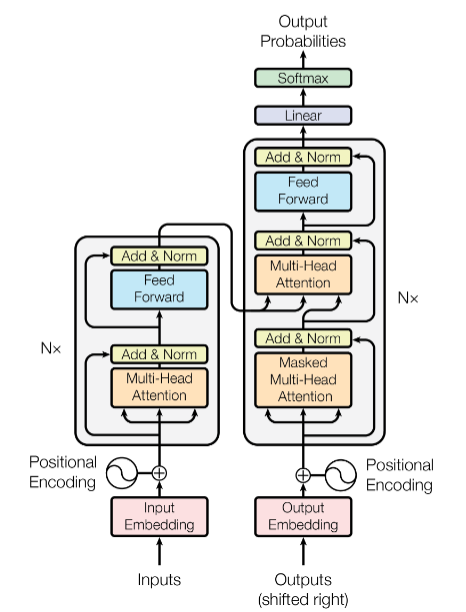
\includegraphics[height=0.75\textheight]{assets/Transformer.png}
		\caption{Transformer Encoder e Decoder}
	\end{figure}
	\column{0.33\textwidth}
	\begin{figure}
		\centering
		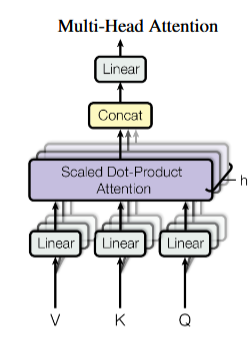
\includegraphics[height=0.75\textheight]{assets/transformer-multi-head-attention.png}
		\caption{Multi-Head Attention}
	\end{figure}
	\column{0.33\textwidth}
	\begin{figure}
		\centering
		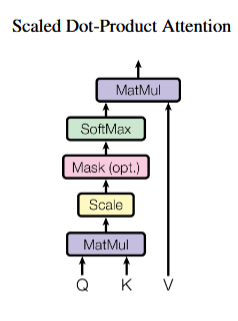
\includegraphics[height=0.75\textheight]{assets/transformer-scaled-dot-attention.png}
		\caption{Multi-Head Attention}
	\end{figure}
\end{columns}
\end{frame}
% 6) Máscara causal e síntese da evolução
\begin{frame}{Resumo da evolução dos modelos}

	\textbf{Linha do tempo (síntese):}
	\begin{itemize}
		\item LSTM encoder--decoder: contexto único $c=h_n$ (gargalo).
		\item LSTM + \textbf{atenção} (Bahdanau/Luong): alívio do gargalo.
		\item \textbf{Self-attention}: dependências longas em paralelo.
		\item \textbf{Transformer}: atenção + posição + FFN; várias camadas empilhadas; sem LSTM.
	\end{itemize}
\end{frame}

\section{Embeddings \& Interpretações}
\begin{frame}{Word/Subword Embeddings}
	\begin{itemize}
		\item Estáticos (Word2Vec, GloVe) vs. Contextuais (ELMo, BERT)
		\item Subword (BPE/Unigram) para robustez morfológica
		\item Análogos em outras modalidades: patches (ViT), time2vec (TS), node2vec (grafos)
	\end{itemize}
\end{frame}

% ---------- Frame 1: Projeções + Compatibilidade + Pesos ----------
\begin{frame}{Atenção: projeções e compatibilidade}
\begin{columns}[t]
  \column{0.55\textwidth}
  \begin{itemize}
    \item \textbf{Projeções lineares}: $Q=XW_Q,\;K=XW_K,\;V=XW_V$.
    \item \textbf{Compatibilidade}: $e_i=\frac{\langle q,k_i\rangle}{\sqrt{d}}$ 
          (ou cosseno se normalizar).
    \item \textbf{Pesos}: $\alpha_i=\mathrm{softmax}(e_i)\Rightarrow \alpha_i\!\ge\!0,\ \sum_i \alpha_i=1$.
  \end{itemize}
  \column{0.45\textwidth}
  \begin{figure}
	\centering
	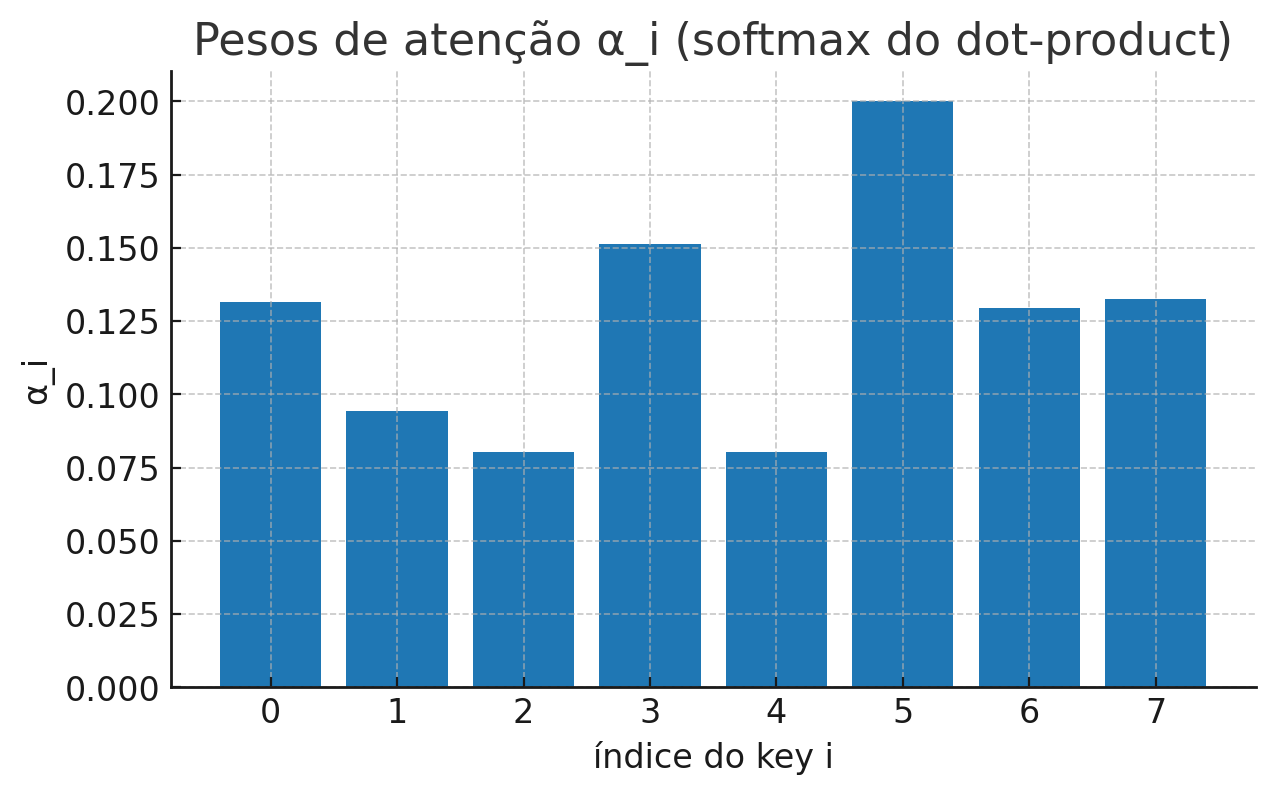
\includegraphics[width=\linewidth]{assets/scalar-softmax.png}
	\caption{Pesos $\alpha_i$ (softmax do dot-product)}
	\end{figure}
\end{columns}
\end{frame}

% ---------- Frame 2: Contexto como combinação convexa ----------
\begin{frame}{Interpretação Geométrica: contexto = barycenter}
\begin{itemize}
  \item \textbf{Contexto}: $c=\sum_i \alpha_i v_i \in \mathrm{conv}\{v_i\}$ 
        $\Rightarrow$ combinação \emph{convexa} dos values.
  \item \textbf{Geometria}: níveis de igual peso são hiperplanos ortogonais a $q$; 
        pesos crescem exponencialmente com o alinhamento entre $q$ e $k_i$.
\end{itemize}
\begin{figure}
	\centering
  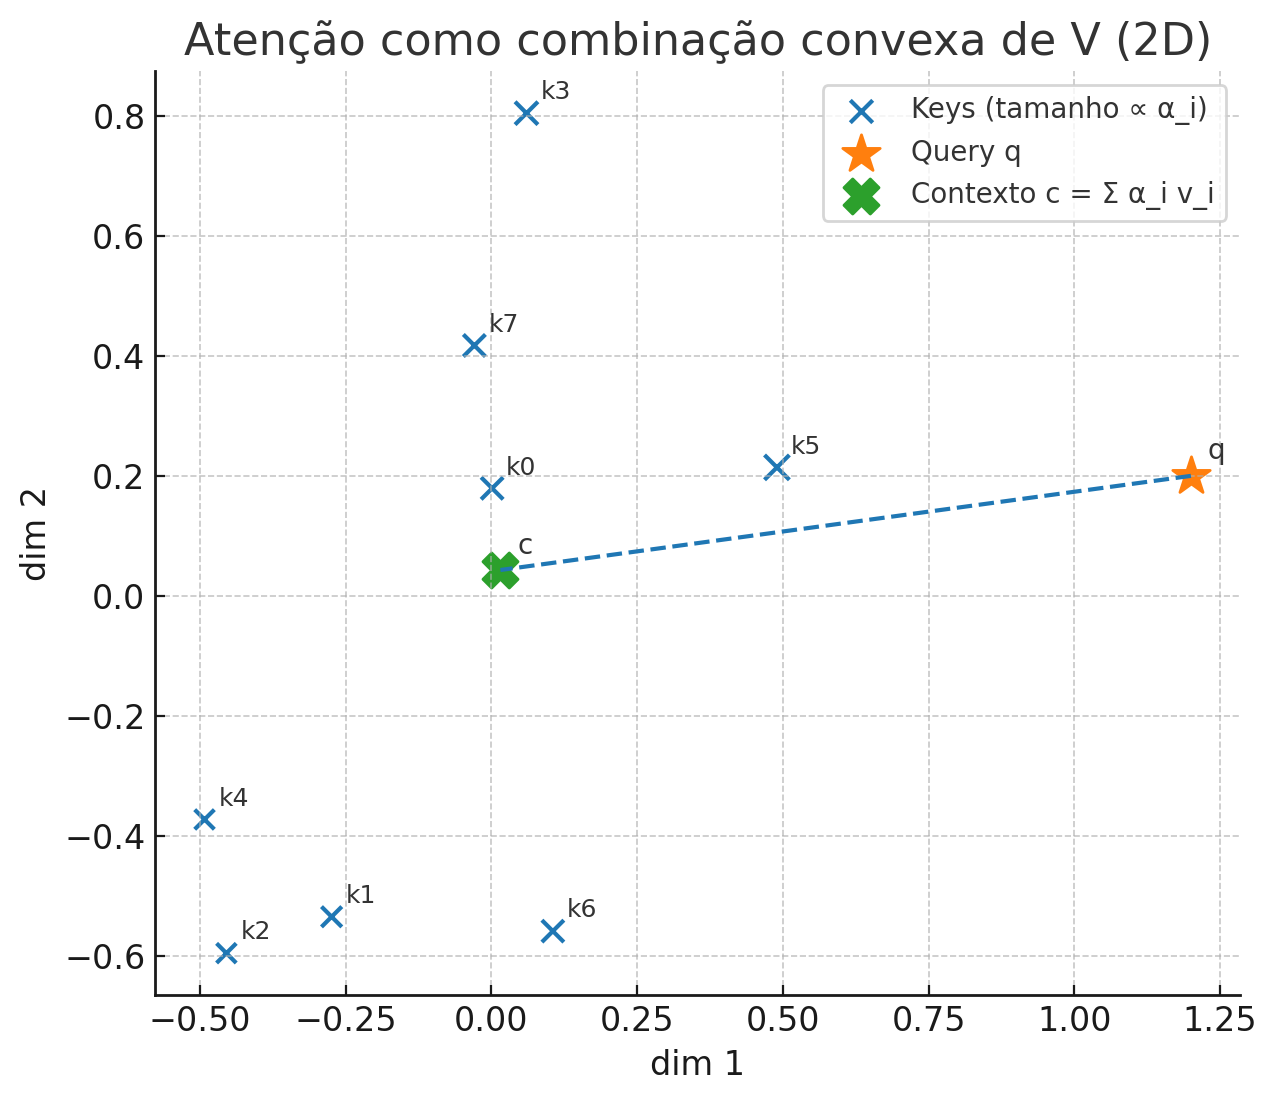
\includegraphics[height=0.7\textheight,keepaspectratio]{assets/rep_2D_cnv.png}
\end{figure}
\end{frame}

% ---------- Frame 3: Multi-head como múltiplas métricas ----------
\begin{frame}{Multi-head: múltiplas projeções/métricas}
\begin{itemize}
  \item Cada head aplica $(W_Q^{(h)},W_K^{(h)},W_V^{(h)})$ e induz 
        uma métrica interna distinta: 
        $\langle x,y\rangle_h = x^\top W_Q^{(h)} {W_K^{(h)}}^\top y$.
  \item Heads diferentes \textrightarrow\ diferentes pesos $\alpha^{(h)}$ e 
        contextos $c^{(h)}$; a saída concatena/combina esses subespaços.
\end{itemize}
\begin{columns}[c]
  \column{0.5\textwidth}
  \begin{figure}
	\centering
	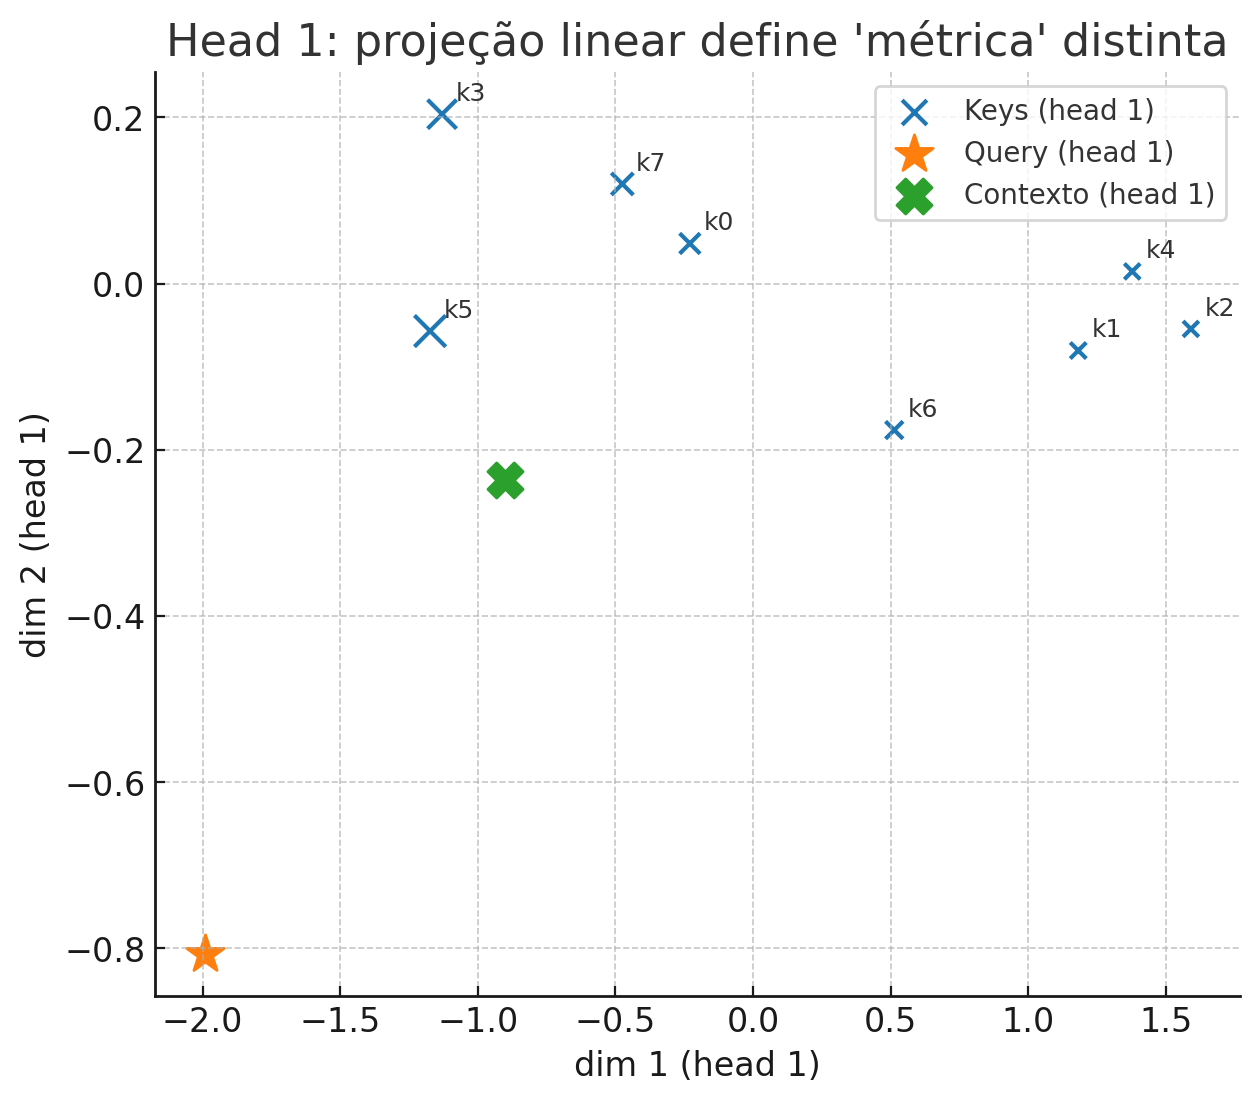
\includegraphics[width=\linewidth,height=0.55\textheight]{assets/att_head1.png}
	\caption{Head 1}
  \end{figure}
  \column{0.5\textwidth}
  \begin{figure}
	\centering
	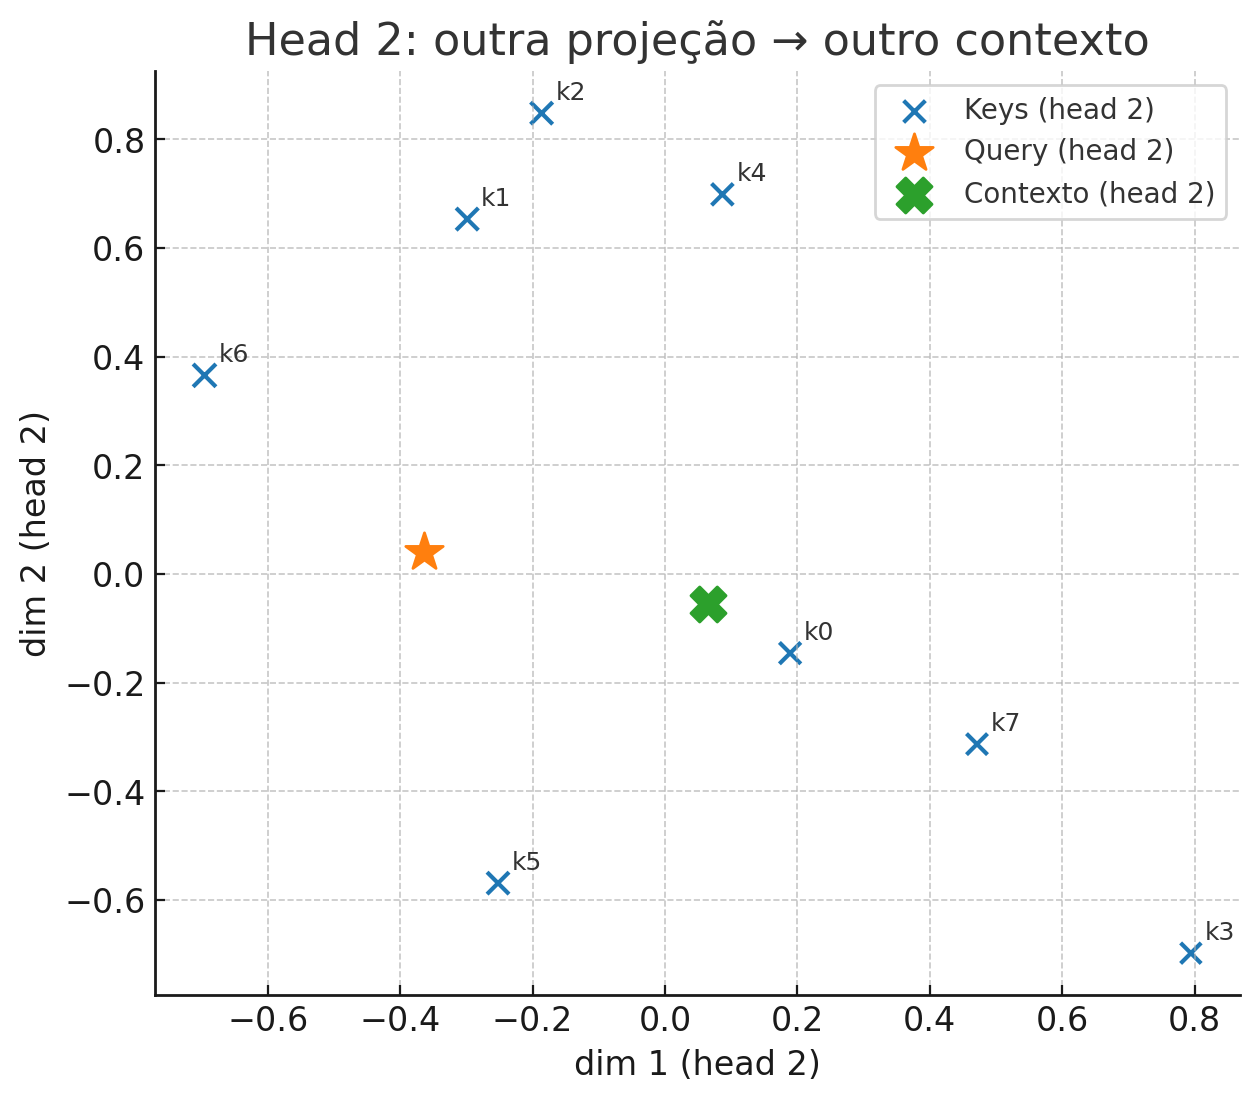
\includegraphics[width=\linewidth,height=0.55\textheight]{assets/att_head2.png}
	\caption{Head 2}
  \end{figure}
\end{columns}
\end{frame}

\begin{frame}{Interpretação Matemática: Self-Attention}
	\begin{block}{Fórmula central (scaled dot-product)}
		\[
			\mathrm{Att}(Q,K,V) \;=\; \mathrm{softmax}\!\left(\frac{QK^\top}{\sqrt{d_k}}\right)\,V
		\]
	\end{block}
	\begin{itemize}
		\item Máscara causal/atencional conforme a tarefa
		\item Complexidade $\mathcal{O}(n^2)$ em tempo/memória
		\item Gradientes e saturação da softmax
	\end{itemize}
\end{frame}

\begin{frame}{Positional Encodings}
	\begin{itemize}
		\item Absolutos senoidais vs. aprendidos
		\item Relativos e RoPE (rotary): melhor generalização/composição
		\item Impacto em extrapolação e contextos longos
	\end{itemize}
\end{frame}

\section{Treino \& Hiperparâmetros}
\begin{frame}{Práticas de Treino}
	\begin{itemize}
		\item AdamW, warmup + decaimento; label smoothing quando aplicável
		\item Regularização: dropout, stochastic depth, weight decay
		\item AMP/mixed precision, grad clipping, checkpointing
		\item Dados: curriculum, masking, augmentation (TS/ViT/GAT)
	\end{itemize}
\end{frame}

\begin{frame}{Hiperparâmetros Essenciais}
	\begin{itemize}
		\item Profundidade, $d_{\text{model}}$, \#heads, $d_{ff}$, dropout
		\item Comprimento de contexto, batch size, \textit{LR schedule}
		\item Específicos: tokenização (LM), \textit{patch size} (ViT), janela/patch (TS)
	\end{itemize}
\end{frame}

\begin{frame}{Qual tamanho ideal? (Scaling)}
\begin{itemize}
  \item \textbf{Leis de escala \cite{kaplan2020scaling}:} 
        desempenho cresce com $\uparrow$ dados, parâmetros e compute, até saturar.
        
  \item \textbf{Trade-offs:} 
        muitos parâmetros + poucos dados $\to$ overfitting; 
        muitos dados + poucos parâmetros $\to$ subutilização.

  \item \textbf{Tokens vs. parâmetros:} 
        ideal quando \#tokens $\approx$ múltiplos de \#parâmetros 
        \cite{hoffmann2022training}.

  \item \textbf{Contexto:} 
        janelas maiores ajudam, mas ganhos saturam.

  \item \textbf{Regra prática:} 
        dimensione conforme dataset + compute + budget de inferência.
\end{itemize}

\vspace{0.2cm}
\textbf{Resumo:} não há tamanho ótimo universal — depende do equilíbrio entre
dados, parâmetros e recursos disponíveis.
\end{frame}



%===========================
% APLICAÇÕES
%===========================

\section{Séries Temporais}
% ------ Frame 1: Explicação ------
\begin{frame}{Atenção em Séries Temporais}
\begin{itemize}
  \item \textbf{Codificação temporal:} absolutos/relativos; \textit{Time2Vec}; embeddings de calendário (hora/dia/sazonalidade).
  \item \textbf{Exógenas + cross-attention:} integrar variáveis externas (clima, preços, feriados) à série-alvo.
  \item \textbf{Contextos longos:} \textit{patching} (janelas), sparsity e hashing; ganhos de janelas muito grandes tendem a saturar.
  \item \textbf{Por que atenção:} foca nos trechos relevantes do histórico e alinha padrões não estacionários/irregulares.
  \item \textbf{Tarefas:} previsão (forecasting), imputação (faltantes) e detecção de anomalias.
\end{itemize}
\end{frame}

% ------ Frame 2: Referências (GitHub) ------
\begin{frame}{Modelos recentes (com código)}
\footnotesize
\begin{itemize}
  \item \href{https://github.com/zhouhaoyi/Informer2020}{Informer (AAAI'21)} — atenção esparsa p/ sequências longas.
  \item \href{https://github.com/thuml/Autoformer}{Autoformer (NeurIPS'21)} — auto-correlação + decomposição.
  \item \href{https://github.com/yuqinie98/PatchTST}{PatchTST (ICLR'23)} — \textit{patching} / channel-independent.
  \item \href{https://github.com/thuml/TimesNet}{TimesNet (ICLR'23)} — modelagem de variação temporal 2D.
  \item \href{https://github.com/natmourajr/CPE883-2025-02/tree/main/models/tsdiffusion}{TSDiffusion (2023)} - difusão para séries temporais.
\end{itemize}
\end{frame}



\section{Language Models}
% ------ Frame 1: Explicação (LMs) ------
\begin{frame}{Language Models (LM)}
\begin{itemize}
  \item \textbf{Atenção causal} (\textit{masked self-attention}): máscara triangular impede olhar o futuro.
  \item \textbf{Objetivo autoregressivo}: minimizar $\;-\sum_{t}\log p(x_t \mid x_{<t})$ (\textit{next-token}).
  \item \textbf{Pré-treino} (corpus amplo, tarefa genérica) \textbf{vs. fine-tuning} (tarefa/estilo): 
        \emph{instruction tuning} (FLAN), RLHF (InstructGPT).
  \item \textbf{PEFT} (ajuste eficiente): \emph{LoRA}, \emph{Adapters} (congelar base + poucos params).
  \item \textbf{Métricas}: 
        \emph{perplexity} (surpresa média por token) e \emph{downstream} (ex.: SuperGLUE, MMLU).
\end{itemize}
\end{frame}
% ------ Frame 2: Referências (links) ------
% ------ Frame 2: Implementações (GitHub) ------
% ------ Frame: Implementações (GitHub) com anos ------
\begin{frame}{Language Models — Implementações (GitHub)}
\scriptsize
\begin{columns}[t]
  \column{0.5\textwidth}
  \begin{itemize}
    \item \href{https://github.com/karpathy/nanoGPT}{karpathy/nanoGPT} \textbf{(2022)} — GPT minimalista
    \item \href{https://github.com/huggingface/transformers}{huggingface/transformers} \textbf{(2019)} — biblioteca SOTA
    \item \href{https://github.com/EleutherAI/gpt-neox}{EleutherAI/gpt-neox} \textbf{(2022)} — treino LLMs em larga escala
    \item \href{https://github.com/meta-llama/llama}{meta-llama/llama} \textbf{(2023)} — código/pesos Llama
    \item \href{https://github.com/harvardnlp/annotated-transformer}{harvardnlp/annotated-transformer} \textbf{(2018)} — Transformer anotado
  \end{itemize}

  \column{0.5\textwidth}
  \begin{itemize}
    \item \href{https://github.com/huggingface/trl}{huggingface/trl} \textbf{(2020)} — SFT, PPO/DPO, RLHF
    \item \href{https://github.com/deepspeedai/DeepSpeedExamples/tree/master/applications/DeepSpeed-Chat}{DeepSpeed-Chat} \textbf{(2023)} — pipeline RLHF
    \item \href{https://github.com/OpenRLHF/OpenRLHF}{OpenRLHF/OpenRLHF} \textbf{(2023)} — RLHF escalável
    \item \href{https://github.com/huggingface/peft}{huggingface/peft} \textbf{(2023)} — PEFT (LoRA, QLoRA, etc.)
    \item \href{https://github.com/adapter-hub/adapters}{adapter-hub/adapters} \textbf{(2020)} — biblioteca de Adapters
    \item \href{https://github.com/microsoft/LoRA}{microsoft/LoRA} \textbf{(2021)} — implementação LoRA oficial
    \item \href{https://github.com/google-research/FLAN}{google-research/FLAN} \textbf{(2021)} — dados p/ instruction tuning
  \end{itemize}
\end{columns}
\end{frame}




\section{Vision Transformer}
\begin{frame}{Vision Transformer (ViT)}
	\begin{itemize}
		\item Imagem $\rightarrow$ \textit{patches} + \texttt{[CLS]} token
		\item Posicionais 2D; augmentations (RandAug, Mixup/CutMix)
		\item Transfer: \textit{linear probe} vs. \textit{fine-tune}
	\end{itemize}
\end{frame}

\section{Graph Attention}
\begin{frame}{Graph Attention Networks (GAT)}
	\begin{block}{Coeficientes de Atenção (um cabeçalho)}
		\small
		\[
			\alpha_{ij}=\mathrm{softmax}_j\!\left(\mathrm{LeakyReLU}\!\big(a^\top[Wh_i \,||\, Wh_j]\big)\right)
		\]
	\end{block}
	\begin{itemize}
		\item Multi-head; sobre-\textit{smoothing} e escalabilidade
		\item Heterógrafos e atenção relacional
	\end{itemize}
\end{frame}

%===========================
% REFERÊNCIAS
%===========================
\section{Referências Bibliográficas}
\begin{frame}[allowframebreaks]
	\frametitle{Referências Bibliográficas}
	\bibliographystyle{ieeetr}
	\bibliography{presentation_bib.bib}
\end{frame}

\end{document}
